\begin{ParaColumn}[\section{Analysis of multivariate clay databases 多元黏土数据库分析}]

    \switchcolumn*[\Paragraph{F-CLAY/7/216 and S-CLAY/7/168 F-CLAY/7/216和S-CLAY/7/168数据库}]
    \switchcolumn*
    
    The first clay database compiled in this study consists of 216 FV data points from 24 different test sites from Finland. Each data “point” contains multivariate information, i.e., information from different tests conducted in close proximity is available. The collected data points contain information on seven basic parameters measured at comparable depths and sampling locations: $s_{\mathrm{u}}^{\mathrm{FV}}, \sigma_{\mathrm{v}}^{\prime},\sigma_{\mathrm{p}}^{\prime}, w, \mathrm{LL}, \mathrm{PL},$ and $S_{\mathrm{t}}$.

    \switchcolumn

    这项研究中汇编的第一个黏土数据库包括来自芬兰24个不同试验点的216个FV数据点。 每个数据“点”都包含多元信息,即,可以使用来自非常接近进行的不同试验的信息。 收集的数据点包含有关在可比较的深度和采样位置处测量的七个基本参数的信息:$s_{\mathrm{u}}^{\mathrm{FV}}, \sigma_{\mathrm{v}}^{\prime},\sigma_{\mathrm{p}}^{\prime}, w, \mathrm{LL}, \mathrm{PL}$和$S_{\mathrm{t}}$。

    \switchcolumn*

    The standard FV test is normally carried out at high speed of rotation, inducing strain rates in the soil that are much higher than in conventional laboratory tests (e.g., triaxial tests, DSS tests). The main consequence is that $s_{u}^{F V}$ is overestimated and, therefore, a correction is needed to convert $s_{u}^{F V}$ into $s_u(\rm{mob})$ (e.g., \citet{Bjerrum19721}). The parameter $s_u(\rm{mob})$ is defined as the undrained shear strength that is mobilized in a full-scale failure of an embankment or slope in the field \citep{Bjerrum19721,Mesri20071}. $s_u(\rm{mob})$ cannot be uniquely defined, as it is a function of failure mode, stress state, and strain rate, among others. In this study, the $s_{u}^{F V}$ values are converted into $s_u(\rm{mob})$ values through a correction factor $\lambda$, as reported in the Finnish Guidelines for stability analysis \citep{Ratahallintokeskus2005}. In this way, rate effects and anisotropy are implicitly accounted for. The strength correction factor used is expressed by \enautoref{equation:9}

    \switchcolumn

    标准FV试验通常在高速旋转下进行,导致土体中的应变率比传统的实验室试验(例如三轴试验,DSS试验)高得多。 主要结果是$s_{u}^{F V}$被高估了,因此需要更正以将$s_{u}^{F V}$转换为$s_u(\rm{mob})$(例如\citet{Bjerrum19721})。 $s_u(\rm{mob})$定义为现场路堤或边坡全面失效时调动的未排水抗剪强度\citep{Bjerrum19721,Mesri20071}。$s_u(\rm{mob})$不能被唯一定义,因为它是失效模式、应力状态和应变率等的函数。 在这项研究中,$s_{u}^{F V}$值通过校正因子$\lambda$转换为$s_u(\rm{mob})$值,如《芬兰稳定性分析指南》\citep{Ratahallintokeskus2005}所述。 这样,就隐含地考虑了速率效应和各向异性。 所使用的强度校正因子由\cnautoref{equation:9}表示。 

    \Equation{
        \begin{align}
            \lambda=\frac{1.5}{1+\mathrm{LL}}
            \label{equation:9}
        \end{align}
    }
    \switchcolumn*
    
    According to \citet{Jamiolkowski198557} and \citet{Chandler198813}, $s_u$ obtained from FV is somewhat comparable to $s_u$ from DSS test results. It is common practice in Sweden to consider su from DSS tests as a reference value (e.g., \citet{Westerberg201577}). DSS tests may, however, be affected by some disturbance effects resulting from sampling as well as specimen preparation. In Finland, DSS tests are not in use and the FV test is normally assumed to provide reliable $s_u$ values, despite some issues related to test equipment. As suggested by \citet{Mansikkamäki2015}, when casing is used to protect the vane during penetration into the ground, rod friction is minimized and, therefore, measured torque values are assumed to be less biased than when slip-coupling is used. FV data points from Finland collected in this study are mostly obtained using FV test equipment that includes casing. As a consequence, the results presented later will likely be representative of the best possible estimate of $s_{u}^{F V}$ in Finnish current practice.

    \switchcolumn

    根据\citet{Jamiolkowski198557}和\citet{Chandler198813}的研究,从FV中获得的$s_u$与DSS试验结果中的$s_u$具有一定的可比性。在瑞典,通常的做法是将来自DSS试验的$s_u$作为参考值(例如,\citet{Westerberg201577})。然而,DSS试验可能会受到取样以及样品制备所产生的一些干扰效应的影响。在芬兰,DSS试验尚未使用,尽管存在一些与试验设备有关的问题,但通常认为FV试验可以提供可靠的$s_u$值。正如\citet{Mansikkamäki2015}所建议的那样,当套管用于保护叶片在插入地面时,杆件摩擦力被最小化,因此,假设测量的扭矩值比使用滑移耦合时的偏差小。本研究中从芬兰收集的FV数据点大多是使用包括套管的FV试验设备获得的。因此,后面介绍的结果很可能代表芬兰目前实践中对$s_{u}^{F V}$的最佳估计。

    \switchcolumn*

    The database is compiled from data given in \citet{Gardemeister1973113}, \citet{Lehtonen2015961}, together with data from recent soil investigations performed by Tampere University of Technology, Finland (J. Selänpää, personal communication, 2015). \citet{Gardemeister1973113} collected FV and oedometer tests performed at different construction sites in Finland. For the purpose of the present study, sites characterized by organic (organic content higher than 2$\%$) and (or) silty soils have been discarded, because the focus of this study is on the strength of inorganic clays. Some low organic clays may, however, be present in the database.

    \switchcolumn

    该数据库是根据\citet{Gardemeister1973113}和\citet{Lehtonen2015961}提供的数据以及芬兰坦佩雷理工大学最近进行的土体调查数据汇编而成(J. Selänpää, personal communication, 2015)。\citet{Gardemeister1973113}收集了在芬兰不同建筑工地进行的FV和固结试验。在本研究中,以有机土(有机含量高于2$\%$)和(或)淤泥质土为特征的场地已被舍弃,因为本研究的重点是无机黏土的强度。然而,数据库中可能存在一些低有机黏土。

    \switchcolumn*

    This database is labeled as F-CLAY/7/216 following the nomenclature proposed by \citeyear{Ching2014663}. F-CLAY/7/216 is a new database that would contribute to the list of multivariate soil databases shown in \enautoref{table:1}. The basic statistics of the seven clay parameters in F-CLAY/7/216 are listed in \enautoref{table:2}. The parameters ${\sigma}_{v}^{\prime}$ and $\sigma_{p}^{\prime}$ are normalized to the atmospheric pressure, $P_a$ ($P_a$ = 101.3 kPa). The numbers of available data points ($n$) are reported in the second column. The statistics shown are the mean value, coefficient of variation (COV), minimum value (Min) and maximum value (Max). Clay properties cover a wide range of $S_t$ values varying from 2 (insensitive clays) to 64 (quick clays), and a wide range of PI values (2$\sim$95) and $w$ values (25$\sim$150).

    \switchcolumn

    根据\citeyear{Ching2014663}提出的命名法,该数据库被标记为F-CLAY/7/216。F-CLAY/7/216是一个新的数据库,将为\cnautoref{table:1}所示的多变量土体数据库列表做出贡献。F-CLAY/7/216中7个黏土参数的基本统计量列于\cnautoref{table:2}中。参数${\sigma}_{v}^{\prime}$和$\sigma_{p}^{\prime}$已归一化为大气压,$P_a$($P_a$ = 101.3 kPa)。可用数据点的数量 ($n$) 在第二栏中显示。显示的统计数据为平均值、变异系数 (COV)、最小值 (Min) 和最大值 (Max)。黏土特性涵盖了从 2(不敏感黏土)到 64(流黏土)的广泛 $S_t$ 值,以及广泛的 PI值(2$\sim$95)和$w$值 (25$\sim$150) 。

    \sidebyside[crosscolumn=true,verticalalignment=bottom][!htb]{0.48\linewidth}{
    \begin{BiliTable}[label=table:2][H]{Basic statistics of the seven basic parameters in F-CLAY/7/216.}{数据库F-CLAY/7/216中七个基本参数的基本统计信息。}
        \tabcolsep=1.5mm
        \begin{tabularx}{\textwidth}{lXXXXX}
            \toprule
            Variable                    & $n$   & Mean   & COV   & Min     & Max\\
            \midrule
            $s_u^{\rm{FV}}\rm{(kPa)}$   & 216   & 21.443 & 0.501 & 5       & 75 \\
            $\sigma_v'/P_a$             & 216   & 0.464  & 0.485 & 0.074   & 1.609 \\
            $\sigma_p'/P_a$             & 216   & 0.948  & 0.515 & 0.251   & 2.884 \\
            LL                          & 216   & 66.284 & 0.298 & 22.0    & 125.0 \\
            PL                          & 216   & 27.740 & 0.204 & 10.0    & 50.0 \\
            $w$                         & 216   & 76.340 & 0.268 & 25.0    & 150.0 \\
            $S_t$                       & 216   & 17.447 & 0.789 & 2.0     & 64.0 \\
            \bottomrule
        \end{tabularx}
    \end{BiliTable}
}{0.48\linewidth}{
    \begin{BiliTable}[label=table:3][H]{Basic statistics of the seven basic parameters in  S-CLAY/7/168.}{数据库S-CLAY/7/168中七个基本参数的基本统计信息。}
        \tabcolsep=1.5mm
        \begin{tabularx}{\textwidth}{lXXXXX}
            \toprule
            Variable                    & $n$   & Mean   & COV   & Min     & Max\\
            \midrule
            $s_u^{\rm{FV}}\rm{(kPa)}$   & 168   & 16.346 & 0.505 & 5.62  & 48.75 \\
            $\sigma_v'/P_a$             & 168   & 0.503  & 0.632 & 0.068 & 2.101 \\
            $\sigma_p'/P_a$             & 168   & 0.786  & 0.726 & 0.15  & 3.116 \\
            LL                          & 168   & 71.055 & 0.396 & 22.77 & 201.81 \\
            PL                          & 168   & 29.448 & 0.344 & 2.73  & 73.92 \\
            $w$                         & 168   & 76.631 & 0.347 & 17.27 & 180.11 \\
            $S_t$                       & 59    & 12.068 & 0.779 & 3.0   & 42.5 \\
            \bottomrule
        \end{tabularx}
    \end{BiliTable}
}

    \switchcolumn*

    A second independent database consisting of 168 FV data points from Sweden and Norway is extracted from the existing global CLAY/10/7490 database \citep{Ching2014663}. This database is labelled as S-CLAY/7/168 and it contains multivariate information on the same soil parameters as in F-CLAY/7/216. The purpose of S-CLAY/7/168 is to act as an independent set of data to be used for comparison with F-CLAY/7/216 in subsequent analyses. The geographical coverage of S-CLAY/7/168 is restricted to Sweden (12 sites) and Norway (seven sites). Full information on all seven parameters is available for only 59 data points. Fortunately, for the remaining 109 data points, information on all six parameters with the exception of $S_t$ is known. The practical implication here is that the effect of $S_t$ on $s_u$ correlations is more difficult to discern in the case of S-CLAY/7/168. Basic statistics of the seven clay parameters in S-CLAY/7/168 are reported in \enautoref{table:3}. The multivariate clay data contained in F-CLAY/7/216 and S-CLAY/7/168 are listed in \enautoref{appendix:a}.

    \switchcolumn

    从现有的全球CLAY/10/7490数据库\citep{Ching2014663}中提取了第二个独立的数据库,其中包括来自瑞典和挪威的168个FV数据点。该数据库被标记为S-CLAY/7/168,包含了与F-CLAY/7/216数据库相同的土体参数的多变量信息。S-CLAY/7/168的目的是作为一套独立的数据,用于在随后的分析中与F-CLAY/7/216进行比较。S-CLAY/7/168的地理范围仅限于瑞典(12个地点)和挪威(7个地点)。只有59个数据点有关于所有七个参数的完整信息。幸运的是,对于其余的109个数据点,除了$S_t$以外,所有六个参数的信息都是已知的。这里的实际意义是,在S-CLAY/7/168的情况下,$S_t$对$s_u$相关性的影响更难辨别。\cnautoref{table:3}为S-CLAY/7/168中7个黏土参数的基本统计。F-CLAY/7/216和S-CLAY/7/168中包含的多变量黏土数据列于\cnautoref{appendix:a}中。

    \switchcolumn*

    \enautoref{figure:1} shows how the data points are positioned in the plasticity chart to provide a broad physical overview of the databases. \enautoref{figure:2} suggests that $w$ tends to increase for increasing LL, and that $w$ is higher than LL for the majority of the data points.

    \switchcolumn

    \cnautoref{figure:1}显示了如何在可塑性图表中定位数据点以提供数据库的广泛物理概览。\cnautoref{figure:2}表明$w$倾向于随着LL的增加而增加,并且对于大多数数据点而言,$w$高于LL。
    
    \sidebyside[crosscolumn=true,verticalalignment=top][!htb]{0.48\linewidth}{
    \begin{BiliFigure}[label=figure:1][H]{Plasticity chart}{塑性图}
        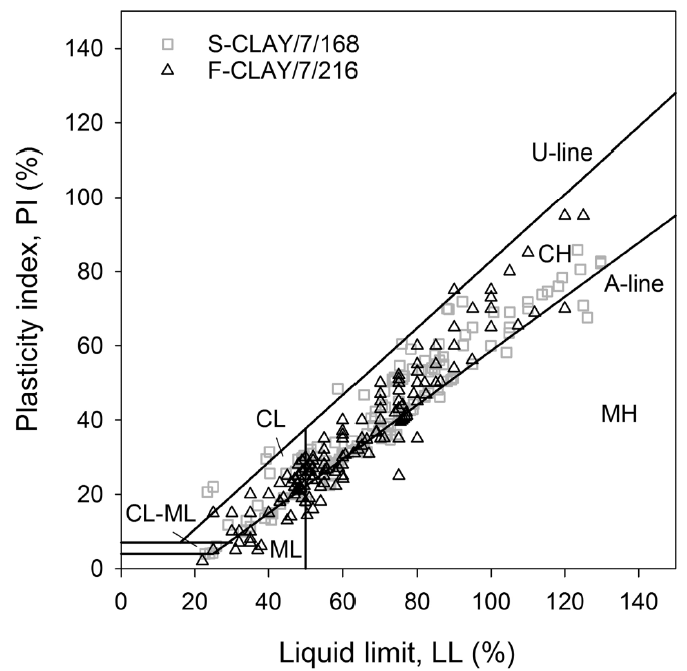
\includegraphics[width=\linewidth]{figures/figure-1.png}
    \end{BiliFigure}
}{0.48\linewidth}{
    \begin{BiliFigure}[label=figure:2][H]{Water content ($w$) versus liquid limit (LL) for F-CLAY/7/216 and S-CLAY/7/168}{F-CLAY/7/216和S-CLAY/7/168的含水量($w$)与液限(LL)}
        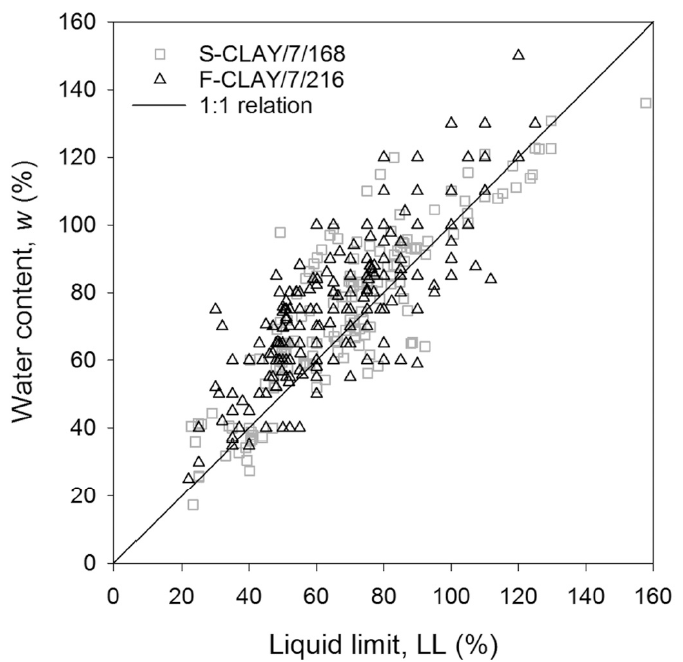
\includegraphics[width=\linewidth]{figures/figure-2.png}
    \end{BiliFigure}
}

    \switchcolumn*[\Paragraph{Dimensionless databases: F-CLAY/10/216 and S-CLAY/10/168 无量纲数据库:F-CLAY/10/216和S-CLAY/10/168}]
    
    Ten dimensionless soil parameters are of primary interest in this study. They are derived from the seven basic clay parameters appearing in F-CLAY/7/216 and S-CLAY/7/168 and they can be categorized into two groups:

    \switchcolumn

    10个无量纲土体参数是本研究的主要内容。它们来自F-CLAY/7/216和S-CLAY/7/168的七个基本黏土参数,可分为两组:

    \switchcolumn*

    \begin{enumerate}
        \item Index properties, including natural water content ($w$), liquid limit (LL), plasticity index (PI), and liquidity index (LI).
        \item Stresses and strengths, including OCR, normalized $s_{\mathrm{u}}(\mathrm{mob})$ against vertical effective stress $\left[s_{\mathrm{u}}(\mathrm{mob}) / \sigma_{\mathrm{v}}^{\prime}\right]$ and preconsolidation pressure $\left[s_{\mathrm{u}}(\mathrm{mob}) / \sigma_{\mathrm{p}}^{\prime}\right]$, normalized $s_{\mathrm{u}}^{\mathrm{FV}}$ against vertical effective stress $\left(s_{\mathrm{u}}^{\mathrm{FV}} / \sigma_{\mathrm{v}}^{\prime}\right)$ and preconsolidation pressure $\left(s_{\mathrm{u}}^{\mathrm{FV}} / \sigma_{\mathrm{p}}^{\prime}\right)$, and sensitivity $\left(S_{\mathrm{t}}=s_{\mathrm{u}} / s_{\mathrm{u}}^{\mathrm{re}}\right)$.
    \end{enumerate}

    \switchcolumn

    \begin{enumerate}
        \item 指数属性,包括天然水含量($w$),液限(LL),塑性指数(PI)和液性指数(LI)。
        \item 应力和强度,包括OCR,针对垂直有效应力$\left[s_{\mathrm{u}}(\mathrm{mob}) / \sigma_{\mathrm{v}}^{\prime}\right]$的归一化$s_{\mathrm{u}}(\mathrm{mob})$和预固结压力$\left[s_{\mathrm{u}}(\mathrm{mob}) / \sigma_{\mathrm{p}}^{\prime}\right]$,针对垂直有效应力$\left(s_{\mathrm{u}}^{\mathrm{FV}} / \sigma_{\mathrm{v}}^{\prime}\right)$的归一化$s_{\mathrm{u}}^{\mathrm{FV}}$,预固结压力$\left(s_{\mathrm{u}}^{\mathrm{FV}} / \sigma_{\mathrm{p}}^{\prime}\right)$和灵敏度$\left(S_{\mathrm{t}}=s_{\mathrm{u}} / s_{\mathrm{u}}^{\mathrm{re}}\right)$。
    \end{enumerate}

    \switchcolumn*

    \enautoref{figure:3a} shows the $s_{u}(\operatorname{mob}) / \sigma_{v}^{\prime}$ values plotted against OCR for F-CLAY/10/216 and S-CLAY/10/168. The trend described by the $s_{\mathrm{u}}(\mathrm{mob}) / \sigma_{\mathrm{v}}^{\prime}$ points vs. OCR seem on average higher for Finnish clays $\mathrm{s}$ than for Scandinavian clays. The reason for such a discrepancy could lie in the definition of $\sigma_{\mathrm{p}}^{\prime}$ used to estimate OCR. Indeed, $\sigma_{\mathrm{p}}^{\prime}$ is normally determined through an oedometer test and it is strongly affected by the strain rate used in the test (e.g., \citet{Leroueil1983477,Leroueil1985159}). As suggested by \citet{Leroueil1985159} and \citet{Leroueil198885,Leroueil1996534}, constant rate of strain (CRS) oedometer tests provide stress-strain curves that normally differ from those provided by conventional 24 h incrementally loaded (IL) oedometer tests. The main reason for such differences can be found in the different rate of loading (or rate of straining) applied during the test. According to \citet{Leroueil1996534}, the strain rate in IL test after 24 h is between $1 \times$ $10^{-7} \mathrm{s}^{-1}$ for highly compressible clays and $5 \times 10^{-8} \mathrm{s}^{-1}$ for low compressible clays. The strain rate in CRS tests is normally between $1 \times$ $10^{-6}-4 \times 10^{-6} \mathrm{s}^{-1} .$ As a consequence, $\sigma_{\mathrm{p}}^{\prime}$ is larger in CRS than in the $24 \mathrm{h}$ IL test \citep{Leroueil1996534}. More specifically, \citet{Leroueil1996534} suggests that $\sigma_{\mathrm{p}}^{\prime}$ obtained from the CRS oedometer test is typically $25 \%$ larger than that deduced from the IL test. For Finnish clays, \citet{Kolisoja198961} reported, for one site in Finland, the ratio $\sigma_{\mathrm{pCRS}}^{\prime} / \sigma_{\mathrm{pIL}}^{\prime}$ to be equal to 1.16. \citet{Hoikkala1991} observed the same ratio to be equal to 1.3 for three different sites in Finland. \citet{Länsivaara1999}, based on the data collected by \citet{Leroueil1996534} on several types of clays, suggested $\sigma_{\text {pCRS }}^{\prime}/\sigma_{\mathrm{pIL}}^{\prime}=1.27 .$ \citet{Karlsrud20131273} observed, for oedometer tests conducted on block samples of Norwegian clays, that $\sigma_{\mathrm{p}}^{\prime}$ values derived from the IL tests were $10 \%-18 \%$ lower than for the CRS tests.

    \switchcolumn

    \cnautoref{figure:3a}显示了针对F-CLAY/10/216和S-CLAY/10/168对OCR的$s_{u}(\operatorname{mob})/\sigma_{v}^{\prime}$值。相对于OCR$s_{\mathrm{u}}(\mathrm{mob})/\sigma_{\mathrm{v}}^{\prime}$点所描述的趋势,芬兰黏土似乎比斯堪的纳维亚黏土平均值较高。出现这种差异的原因可能在于用于估计OCR的$\sigma_{\mathrm{p}}^{\prime}$的定义。实际上,$\sigma_{\mathrm{p}}^{\prime}$通常是通过固结试验确定的,并且受试验中使用的应变率的强烈影响(例如\citet{Leroueil1983477,Leroueil1985159})。如\citet{Leroueil1985159}和\citet{Leroueil198885,Leroueil1996534}所建议,恒定应变率(CRS)固结试验提供的应力-应变曲线通常不同于传统的24小时增量加载(IL)固结试验提供的应力-应变曲线。这种差异的主要原因可以在试验过程中施加的不同加载速率(或应变速率)中找到。根据\citet{Leroueil1996534}的研究,对于高度可压缩的黏土IL试验24小时后的应变率在$1\times 10^{-7}\mathrm{s}^{-1}$之间,而低压缩性黏土为$5\times 10^{-8}\mathrm{s}^{-1}$。CRS试验中的应变率通常在$1\times 10^{-6}$到$4\times 10^{-6}\mathrm{s}^{-1}$之间。因此,CRS中的$\sigma_{\mathrm{p}}^{\prime}$比24小时的IL试验中的要大\citep{Leroueil1996534}。更具体地说,\citet{Leroueil1996534}提出,从CRS固结试验获得的$\sigma_{\mathrm{p}}^{\prime}$通常比从IL试验得出的值大25$\%$。对于芬兰黏土,\citet{Kolisoja198961}报告,对于芬兰的一个站点,比率$\sigma_{\mathrm{pCRS}}^{\prime}/\sigma_{\mathrm{pIL}}^{\prime}$等于1.16。\citet{Hoikkala1991}观察到芬兰三个不同地点的比率均等于1.3。\citet{Länsivaara1999}根据\citet{Leroueil1996534}收集的关于几种类型黏土的数据,提出了$\sigma_{\text{pCRS}}^{\prime}/\sigma_{\mathrm{pIL}}^{\prime}=1.27$。\citet{Karlsrud20131273}在对挪威黏土块状样品进行的固结试验中观察到,来自IL试验的$\sigma_{\mathrm{p}}^{\prime}$值比CRS试验低$10\%-18\%$。

    \switchcolumn*

    Upon examination of the original sources (listed in Table $A1$ of \citet{Ching2014663}) from where data contained in S-CLAY/ $7 / 168$ have been collected, it seems that $\sigma_{\mathrm{p}}^{\prime}$ points were mostly measured from CRS oedometer tests. F-CLAY/7/216 contains only 56 $\sigma_{\mathrm{pCRS}}^{\prime}$ points, while the remaining 162 points are from 24h $\mathrm{IL}$ tests $\left(\sigma_{\mathrm{pI}}^{\prime}\right)$ (\enautoref{figure:3a}). Therefore, to make data suitable for comparison, $\sigma_{\mathrm{pIL}}^{\prime}$ is increased by $27\%$ for all data points as a first-order correction following the proposal by \citet{Länsivaara1999} (\enautoref{figure:3b}). By applying $\sigma_{\mathrm{pCRS}}^{\prime} / \sigma_{\mathrm{pll}}^{\prime}=1.27$ to all $162 \sigma_{\mathrm{plL}}^{\prime}$ values from Finland, the strength points from F-CLAY/10/216 seem to better adapt to the $s_{y}(\mathrm{mob}) / \sigma_{\mathrm{v}}^{\prime}-\mathrm{OCR}$ trend shown by those contained in S-CLAY/10/168 (\enautoref{figure:3b}). It is plausible that the difference between F-CLAY/7/216 and S-CLAY/10/168 in the $s_{\mathrm{u}}(\mathrm{mob}) / \sigma_{\mathrm{v}}^{\prime}$ versus $\mathrm{OCR}$ plot is primarily caused by the difference between the CRS and IL test, rather than the difference between clay types, as also indicated by \enautoref{figure:1} and \enautoref{figure:1}.

    \switchcolumn
    
    在检查原始来源(列于\citet{Ching2014663}的表A1)后,从中收集了S-CLAY/7/168的数据,似乎$\sigma_{\mathrm{p}}^{\prime}$点主要是通过CRS固结试验测得的。F-CLAY/7/216仅包含56个$\sigma_{\mathrm{pCRS}}^{\prime}$点,其余162个点来自24小时IL试验$\left(\sigma_{\mathrm{pI}}^{\prime}\right)$(\cnautoref{figure:3a})。 因此,为了使数据适合比较,按照\citet{Länsivaara1999}的建议(\cnautoref{figure:3b}),对所有数据点的$\sigma_{\mathrm{pIL}}^{\prime}$增加$27\%$作为一阶校正。 通过对芬兰的所有162个$\sigma_{\mathrm{pIL}}^{\prime}$值应用$\sigma_{\mathrm{pCRS}}^{\prime} / \sigma_{\mathrm{pll}}^{\prime}=1.27$,F-CLAY/10/216的数据点似乎要比S-CLAY/10/168(\cnautoref{figure:3b})的数据点更好地适应$s_{y}(\mathrm{mob}) / \sigma_{\mathrm{v}}^{\prime}-\mathrm{OCR}$显示的趋势。  $s_{y}(\mathrm{mob}) / \sigma_{\mathrm{v}}^{\prime}-\mathrm{OCR}$图中的F-CLAY/10/216和S-CLAY/10/168之间的差异可能主要是由CRS和IL试验之间的差异引起的,而不是由黏土类型之间的差异,也正如\cnautoref{figure:1}和\cnautoref{figure:2}所示。

    \switchcolumn*

    The basic statistics of the 10 dimensionless parameters are listed in \enautoref{table:4} and \enautoref{table:5} for the dimensionless databases, labeled as F-CLAY/10/216 and S-CLAY/10/168, respectively.

    \switchcolumn

    \cnautoref{table:4}和\cnautoref{table:5}中列出了针对无量纲数据库的10个无量纲参数的基本统计信息,分别标记为F-CLAY/10/216和S-CLAY/10/168。
   
    \begin{BiliFigure}[crosscolumn=true,label=figure:3][!htb]{$s_{\mathrm{u}}(\mathrm{mob}) / \sigma_{\mathrm{v}}^{\prime}$ against OCR}{$s_{\mathrm{u}}(\mathrm{mob}) / \sigma_{\mathrm{v}}^{\prime}$与OCR的关系}
    \subfigure[raw data point]{
        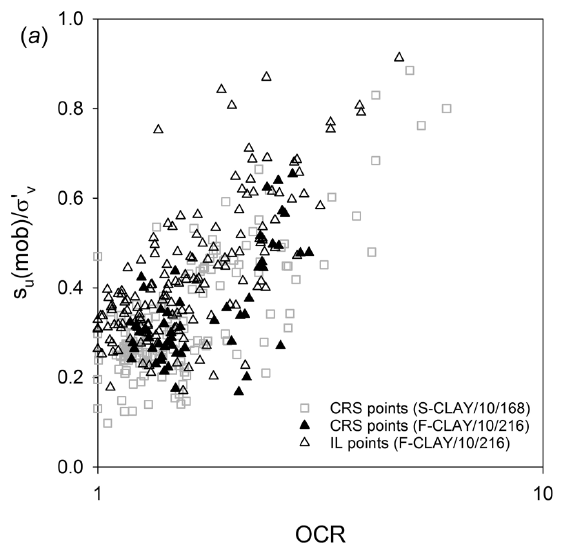
\includegraphics[width=0.48\linewidth]{figures/figure-3a.png}
        \label{figure:3a}
    }
    \subfigure[data points corrected to $\sigma_{\mathrm{p}}^{\prime}$ from CRS oedometer test using $\sigma_{\mathrm{pCRS}}^{\prime} / \sigma_{\mathrm{pIL}}^{\prime}=1.27$]{
        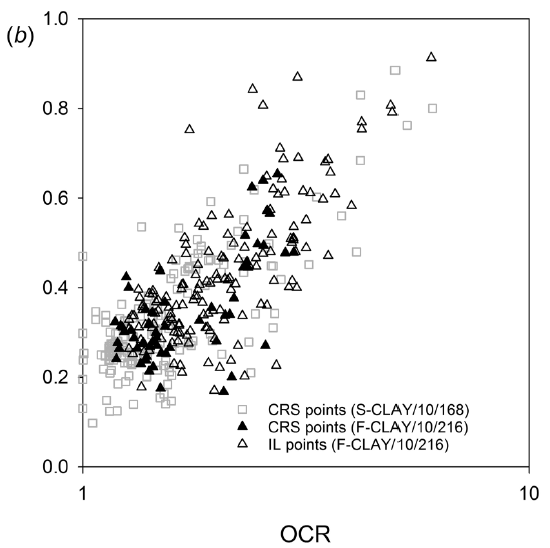
\includegraphics[width=0.48\linewidth]{figures/figure-3b.png}
        \label{figure:3b}
    }
\end{BiliFigure}
    \sidebyside[crosscolumn=true,verticalalignment=bottom][!htb]{0.49\linewidth}{
    \begin{BiliTable}[label=table:4][H]{Basic statistics of 10 dimensionless soil parameters in F-CLAY/10/216, derived from the seven basic parameters in F-CLAY/7/216.}{从F-CLAY/7/216中的七个基本参数得出的F-CLAY/10/216中10个无量纲土体参数的基本统计信息}
        \tabcolsep=1.5mm
        \begin{tabularx}{\textwidth}{lXXXXX}
            \toprule
            Variable                    & $n$   & Mean   & COV   & Min   & Max \\
            \midrule
            $s_u(\rm{mob})/\sigma_v'$   & 168   & 0.329 & 0.417  & 0.098 & 0.885 \\
            $s_u(\rm{mob})/\sigma_p'$   & 168   & 0.21  & 0.269  & 0.088 & 0.470 \\
            $s_u^{\rm{FV}}/\sigma_v'$   & 168   & 0.386 & 0.469  & 0.098 & 0.974 \\
            $s_u^{\rm{FV}}/\sigma_p'$   & 168   & 0.244 & 0.311  & 0.088 & 0.490 \\
            OCR                         & 168   & 1.664 & 0.476  & 1.00  & 6.07 \\
            LL                          & 168   & 71.06 & 0.396  & 22.77 & 201.81 \\
            PI                          & 168   & 41.61 & 0.496  & 3.91  & 127.89 \\
            w                           & 168   & 76.63 & 0.347  & 17.27 & 180.11 \\
            LI                          & 168   & 1.267 & 0.507  & 0.60  & 5.50 \\
            St                          & 59    & 12.068 & 0.779 & 3.00  & 42.50 \\
            \bottomrule
        \end{tabularx}
    \end{BiliTable}
}{0.49\linewidth}{
    \begin{BiliTable}[label=table:5][H]{Basic statistics of 10 dimensionless soil parameters in F-CLAY/10/168, derived from the seven basic parameters in F-CLAY/7/168}{从F-CLAY/7/168中的七个基本参数得出的F-CLAY/10/168中10个无量纲土体参数的基本统计信息}
        \tabcolsep=1.5mm
        \begin{tabularx}{\textwidth}{lXXXXX}
            \toprule
            Variable                    & $n$   & Mean   & COV   & Min   & Max \\
            \midrule
            $s_u(\rm{mob})/\sigma_v'$   & 216   & 0.458  & 0.715 & 0.167 & 2.754 \\
            $s_u(\rm{mob})/\sigma_p'$   & 216   & 0.209  & 0.281 & 0.081 & 0.469 \\
            $s_u^{\rm{FV}}/\sigma_v'$   & 216   & 0.513  & 0.712 & 0.176 & 2.938 \\
            $s_u^{\rm{FV}}/\sigma_p'$   & 216   & 0.234  & 0.293 & 0.083 & 0.594 \\
            OCR                         & 216   & 2.17   & 0.467 & 1.18  & 7.50  \\
            LL                          & 216   & 66.284 & 0.298 & 22.0  & 125.0 \\
            PI                          & 216   & 38.545 & 0.482 & 2.0   & 95.0  \\
            $w$                         & 216   & 76.34  & 0.268 & 25.0  & 150.0 \\
            LI                          & 216   & 1.443  & 0.459 & 0.425 & 4.800 \\
            $S_t$                          & 216   & 17.447 & 0.789 & 2.0   & 64.0  \\
            \bottomrule
        \end{tabularx}
    \end{BiliTable}
}

    \switchcolumn*[\Paragraph{Comparison with existing transformation models 与现有转换模型的比较}]
    
    The 384 clay data points constituting F-CLAY/10/216 and S-CLAY/10/168 databases are compared with transformation models proposed in the literature to check their consistency. It is worth pointing out that transformation models are generally derived based on certain types of clays and geographical locations. The basis for these models is usually empirical. Very often, for such models we do not know the basic statistics (such as those reported in \enautoref{table:4} and \enautoref{table:5} ).

    \switchcolumn

    将构成F-CLAY/10/216数据库和S-CLAY/10/168数据库的384个黏土数据点与文献中提出的转换模型进行比较,以检查其一致性。 值得指出的是,转换模型通常是基于某些类型的黏土和地理位置得出的。 这些模型的基础通常是经验性的。 通常,对于此类模型,我们不了解基本统计信息(例如\cnautoref{table:4}和\cnautoref{table:5}中报告的统计信息)。

    \switchcolumn*

    The 10 transformation models analyzed are labeled using the following template: "primary input parameter" - "target parameter" - "secondary input parameter". They are categorized into four types (see e.g., \enautoref{table:6}):

    \switchcolumn
        
    使用以下模板标记分析的10个转换模型:“主要输入参数”-“目标参数”“次要输入参数”。 它们分为四种类型(例如,参见\cnautoref{table:6}):

    \newcommand{\RelationshipAA}{$\rm{LI}-s_u^{re}/P_a$}
\newcommand{\RelationshipAB}{$\rm{LI}-S_t$}
\newcommand{\RelationshipBA}{$\rm{LI}-(\sigma_p'/P_a)-S_t(\rm{for}~S_t<15)$}
\newcommand{\RelationshipBB}{$\rm{LI}-(\sigma_p'/P_a)-S_t(\rm{for}~S_t>15)$}
\newcommand{\RelationshipCA}{$\rm{PI}-s_u(\rm{mob})/\sigma_p'$}
\newcommand{\RelationshipCB}{$\rm{OCR}-s_u(\rm{mob})/\sigma_v'$}
\newcommand{\RelationshipCC}{$\rm{OCR}-s_u(\rm{mob})/\sigma_v'-S_t$}
\newcommand{\RelationshipDA}{$\rm{LL}-(s_u^{\rm{FV}}/\sigma_p')$}
\newcommand{\RelationshipDB}{$\rm{PI}-(s_u^{\rm{FV}}/\sigma_p')$}

\newcommand{\LiteratureAA}{\citet{Wroth1978137}}
\newcommand{\LiteratureAB}{\citet{Locat1988799}}
\newcommand{\LiteratureAC}{\citet{Bjerrum195449}}
\newcommand{\LiteratureAD}{\citet{Ching2012522}}
\newcommand{\LiteratureBA}{\citet{Ching2012522}}
\newcommand{\LiteratureBB}{\citet{Ching2012522}}
\newcommand{\LiteratureCA}{\citet{Mesri1975409,Mesri1989162}}
\newcommand{\LiteratureCB}{\citet{Jamiolkowski198557}}
\newcommand{\LiteratureCC}{\citet{Ching2012522}}
\newcommand{\LiteratureDA}{\citet{Hansbo1957}}
\newcommand{\LiteratureDB}{\citet{Larsson1980591}}
\newcommand{\LiteratureDC}{\citet{Chandler198813}}

\newcommand{\ModelAA}{$s_u^{re}/P_a\approx{}1.7^{-4.6\rm{LI}}$}
\newcommand{\ModelAB}{$s_u^{re}/P_a\approx{}0.0144\rm{LI}^{-2.44}$}
\newcommand{\ModelAC}{$S_t\approx10^{0.8\rm{LI}}$}
\newcommand{\ModelAD}{$S_t\approx{}20.726\rm{LI}^{1.910}$}
\newcommand{\ModelBA}{$\sigma_p'/P_a\approx{}0.235\rm{LI}^{-1.139}S_t^{0.536}$}
\newcommand{\ModelBB}{$\sigma_p'/P_a\approx{}0.235\rm{LI}^{-1.139}S_t^{0.536}$}
\newcommand{\ModelCA}{$s_u(\rm{mob})/\sigma_p'\approx{}0.22$}
\newcommand{\ModelCB}{$s_u(\rm{mob})/\sigma_v'\approx{}0.23\rm{OCR}^{0.8}$}
\newcommand{\ModelCC}{$s_u(\rm{mob})/\sigma_p'\approx{}0.229\rm{OCR}^{0.823}S_t^{0.121}$}
\newcommand{\ModelDA}{$s_u^{\rm{FV}}/\sigma_p'\approx{}0.45\rm{LI}$}
\newcommand{\ModelDB}{$s_u^{\rm{FV}}/\sigma_p'\approx{}0.08+0.0055\rm{PI}$}
\newcommand{\ModelDC}{$s_u^{\rm{FV}}/\sigma_p'\approx{}0.11+0.0037\rm{PI}$}


\begin{BiliTable}[crosscolumn=true,label=table:6][!htb]{Transformation models in literature and their calibration results for F-CLAY/10/216}{文献中的转换模型及其对F-CLAY/10/216的校准结果}
    \footnotesize
    \tabcolsep=0.3mm
    \begin{tabular}{lllllllll}
        \toprule
                &                 &               &      &         & \multicolumn{2}{l}{Comprasion} & \multicolumn{2}{l}{Calibration} \\
        Type    & Relationship    & Literature    & $n$  & Transformation model & Figure & \makecell[l]{Fit to\\trend?} & \makecell{Bias\\factor,b} & \makecell{COV of\\$\varepsilon=\delta$}\\
        \midrule
        A       & \RelationshipAA & \LiteratureAA & 899  & \ModelAA &  Fig.\ref{figure:9}      & NO       & $-$        & $-$ \\
                &                 & \LiteratureAB & 899  & \ModelAB &  Fig.\ref{figure:9}      & YES      & 4.05      & 3.02 \\
                & \RelationshipAB & \LiteratureAC & 1279 & \ModelAC &  Fig.\ref{figure:11}     & YES      & 1.56      & 1.40 \\
                &                 & \LiteratureAD & 1279 & \ModelAD &  Fig.\ref{figure:11}     & NO       & 0.57      & 1.94 \\
        B       & \RelationshipBA & \LiteratureBA & 694  & \ModelBA &  Fig.\ref{figure:12a}    & YES      & 2.02      & 0.94 \\
                & \RelationshipBB & \LiteratureBB & 492  & \ModelBB &  Fig.\ref{figure:12a}    & YES      & 0.95      & 0.47 \\
        C       & \RelationshipCA & \LiteratureCA & 1072 & \ModelCA &  Fig.\ref{figure:5}      & YES      & 0.95      & 0.28 \\
                & \RelationshipCB & \LiteratureCB & 1155 & \ModelCB &  Fig.\ref{figure:6}      & YES      & 1.06      & 0.30 \\
                & \RelationshipCC & \LiteratureCC & 1402 & \ModelCC &  Fig.\ref{figure:6a}     & YES      & 0.77      & 0.32 \\
        D       & \RelationshipDA & \LiteratureDA & 423  & \ModelDA &  Fig.\ref{figure:7}      & YES      & 0.84      & 0.38 \\
                & \RelationshipDB & \LiteratureDB & 428  & \ModelDB &  Fig.\ref{figure:8}      & YES      & 0.89      & 0.43 \\
                &                 & \LiteratureDC & 423  & \ModelDC &  Fig.\ref{figure:8}      & YES      & 0.97      & 0.35 \\
        \bottomrule
    \end{tabular}
\end{BiliTable}
    \switchcolumn*

    Type A: Models for $S_{\mathrm{t}}$, including two $\mathrm{LI}-\left(s_{\mathrm{u}}^{\mathrm{re}} / P_{\mathrm{a}}\right)$ models and two $\mathrm{LI}-\left(S_{\mathrm{t}}\right)$ models.
 
    Type B:  Models for effective stress, including one $\mathrm{LI}-\left(\sigma_{p}^{\prime} / P_{a}\right)-S_{t}$ model. Basic statistics of $\sigma_{\mathrm{p}}^{\prime} / \mathrm{P}_{\mathrm{a}}$ are reported in \enautoref{table:2} and \enautoref{table:3} and not included in the dimensionless databases, as $s_{\mathrm{u}}^{\mathrm{FV}}$ and $s_{\mathrm{u}}(\mathrm{mob})$ are the parameters of primary interest for this study. 
    
    Type C: Models for shear strength, including one $\mathrm{PI}-\left[\mathrm{s}_{\mathrm{u}}(\mathrm{mob}) / \sigma_{\mathrm{p}}^{\prime}\right]$ model, one $\mathrm{OCR}-\left[s_{\mathrm{u}}(\mathrm{mob}) / \sigma_{\mathrm{v}}^{\prime}\right]$ model, and one $\mathrm{OCR}-\left[\mathrm{s}_{\mathrm{u}}(\mathrm{mob}) / \sigma_{\mathrm{v}}^{\prime}\right]-S_{\mathrm{t}}$ model. 
    
    Type D: Models for shear strength, including two $\mathrm{PI}-\left(s_{\mathrm{u}}^{\mathrm{FV}} / \sigma_{\mathrm{p}}^{\prime}\right)$ one $\mathrm{LL}-\left(s_{\mathrm{u}}^{\mathrm{FV}} / \sigma_{\mathrm{p}}^{\prime}\right)$. These three models are compared to uncorrected $s_{\mathrm{u}}^{\mathrm{FV}}$($\lambda$ correction factor is not applied), being originally derived from uncorrected measurements.

    \switchcolumn

    A类:$S_t$的模型,包括两个$\mathrm{LI}-\left(s_{\mathrm{u}}^{\mathrm{re}} / P_{\mathrm{a}}\right)$模型和两个$\mathrm{LI}-\left(S_{\mathrm{t}}\right)$模型。
  
    B类:有效应力的模型,包括一个$\mathrm{LI}-\left(\sigma_{p}^{\prime} / P_{a}\right)-S_{t}$模型。  $\sigma_{\mathrm{p}}^{\prime} / \mathrm{P}_{\mathrm{a}}$的基本统计数据在\cnautoref{table:2}和\cnautoref{table:3}中报告,并且不包含在无量纲数据库中,因为$s_{\mathrm{u}}^{\mathrm{FV}}$和$s_{\mathrm{u}}(\mathrm{mob})$是这项研究的主要参数。
   
    C类:剪切强度的模型,包括一个$\mathrm{PI}-\left[\mathrm{s}_{\mathrm{u}}(\mathrm{mob}) / \sigma_{\mathrm{p}}^{\prime}\right]$,一个$\mathrm{OCR}-\left[s_{\mathrm{u}}(\mathrm{mob}) / \sigma_{\mathrm{v}}^{\prime}\right]$模型和一个$\mathrm{OCR}-\left[\mathrm{s}_{\mathrm{u}}(\mathrm{mob}) / \sigma_{\mathrm{v}}^{\prime}\right]-S_{\mathrm{t}}$模型。
   
    D类:剪切强度的模型,包括两个$\mathrm{PI}-\left(s_{\mathrm{u}}^{\mathrm{FV}} / \sigma_{\mathrm{p}}^{\prime}\right)$,一个$\mathrm{LL}-\left(s_{\mathrm{u}}^{\mathrm{FV}} / \sigma_{\mathrm{p}}^{\prime}\right)$模型。 将这三个模型与未经修正的$s_{\mathrm{u}}^{\mathrm{FV}}$($\lambda$修正因子未应用)进行比较,该模型最初是由未经修正的测量得出的。

    \switchcolumn*

    Many of the transformation models are derived empirically using regression analyses. Only the $\mathrm{LI}-\left(s_{\mathrm{u}}^{\mathrm{re}} / P_{\mathrm{a}}\right)$ model by \citet{Wroth1978137} represents an exception. It is derived theoretically from the modified Cam clay model. The $\mathrm{LI}-\left(\sigma_{\mathrm{p}}^{\prime} / \mathrm{P}_{\mathrm{a}}\right)-S_{\mathrm{t}}$ and $\mathrm{OCR}-\left[s_{u}(\operatorname{mob}) / \sigma_{v}^{\prime}\right]-S_{t}$ models proposed by \citet{Ching2012522} are derived from sensitive structured clay data. The $\mathrm{LI}-S_{\mathrm{t}}$ model by \citet{Bjerrum195449} is based on Norwegian marine clay data.

    \switchcolumn

    许多转换模型是使用回归分析根据经验得出的。 只有\citet{Wroth1978137}的$\mathrm{LI}-\left(s_{\mathrm{u}}^{\mathrm{re}} / P_{\mathrm{a}}\right)$模型代表例外。 它是从理论上从改进的Cam clay模型得出的。\citet{Ching2012522}提出的$\mathrm{LI}-\left(\sigma_{\mathrm{p}}^{\prime} / \mathrm{P}_{\mathrm{a}}\right)-S_{\mathrm{t}}$和$\mathrm{OCR}-\left[s_{u}(\operatorname{mob}) / \sigma_{v}^{\prime}\right]-S_{t}$模型是从敏感的结构化黏土数据中得出的。\citet{Bjerrum195449}的$\mathrm{LI}-S_{\mathrm{t}}$模型基于挪威海洋黏土数据。

    \sidebyside[crosscolumn=true][p]{0.45\textwidth}{
    \begin{BiliFigure}[label=figure:4][H]{$\mathrm{OCR}-\left[s_{u}(mob)/\sigma_{v}^{\prime}\right]$ model proposed by \citet{Jamiolkowski198557}}{\citet{Jamiolkowski198557}提出的$\mathrm{OCR}-\left[s_{u}(mob)/\sigma_{v}^{\prime}\right]$模型}
        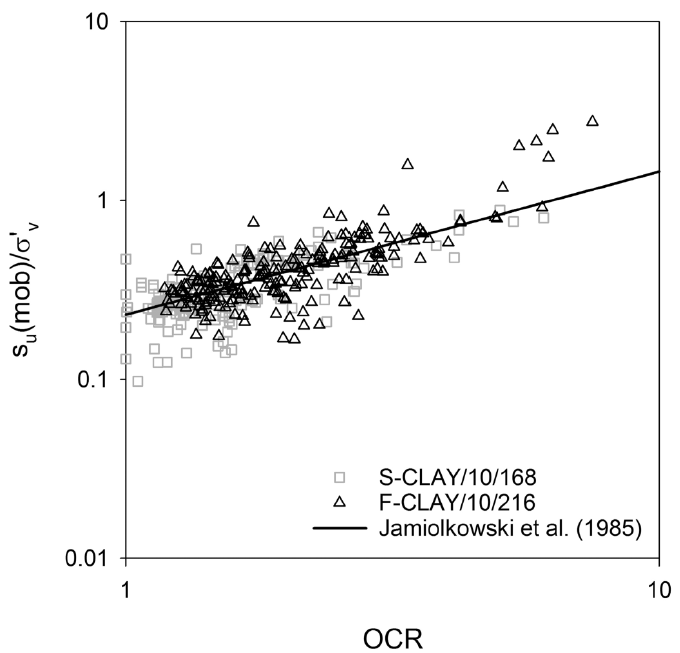
\includegraphics[width=\textwidth]{figures/figure-4.png}
    \end{BiliFigure}
}{0.48\textwidth}{
    \begin{BiliFigure}[label=figure:5][H]{$\mathrm{PI}-\left[s_{\mathrm{u}}(\mathrm{mob})/\sigma_{\mathrm{p}}^{\prime}\right]$ model proposed by \citet{Mesri1975409,Mesri1989162}}{\citet{Mesri1975409,Mesri1989162}提出的$\mathrm{PI}-\left[s_{\mathrm{u}}(\mathrm{mob}) / \sigma_{\mathrm{p}}^{\prime}\right]$模型}
        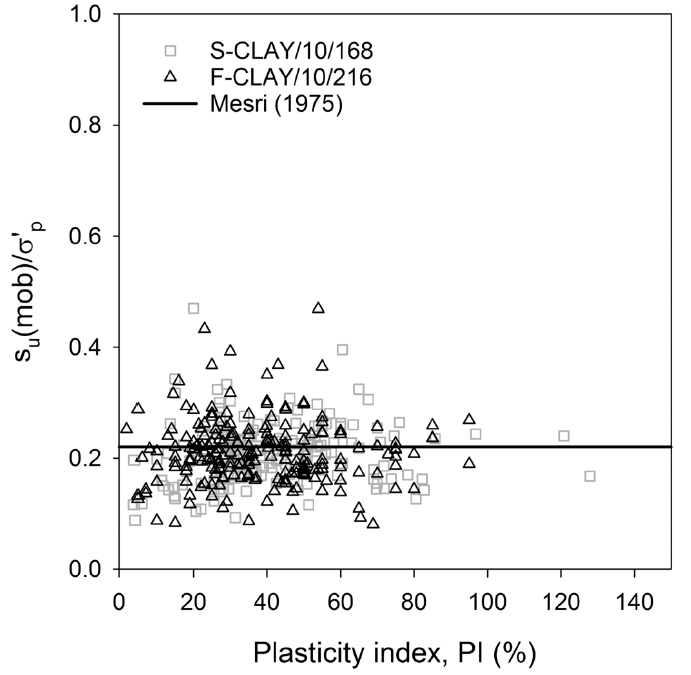
\includegraphics[width=\textwidth]{figures/figure-5.png}
    \end{BiliFigure}
}

    \begin{BiliFigure}[crosscolumn=true,label=figure:6][p]{$\mathrm{OCR}-\left[\mathrm{s}_{\mathrm{u}}(\mathrm{mob}) / \sigma_{\mathrm{v}}^{\prime}\right]-S_{\mathrm{t}}$ model proposed by \citet{Ching2012522}}{\citet{Ching2012522}提出的$\mathrm{OCR}-\left[\mathrm{s}_{\mathrm{u}}(\mathrm{mob}) / \sigma_{\mathrm{v}}^{\prime}\right]-S_{\mathrm{t}}$模型}
    \subfigure[F-CLAY/10/216]{
        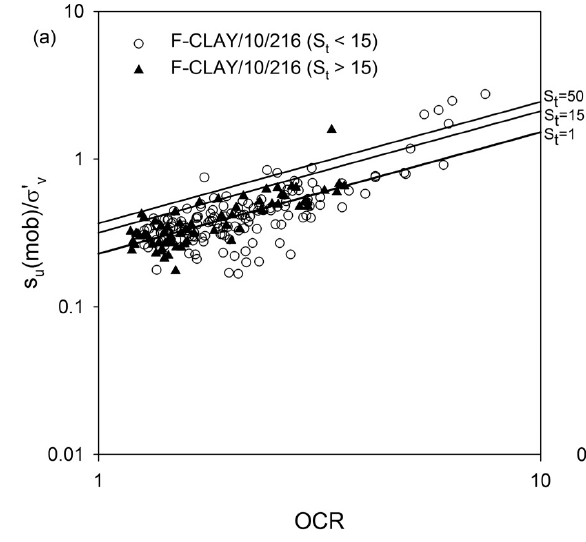
\includegraphics[width=0.48\textwidth]{figures/figure-6a.png}
        \label{figure:6a}
    }
    \hspace{\fill}
    \subfigure[S-CLAY/10/168]{
        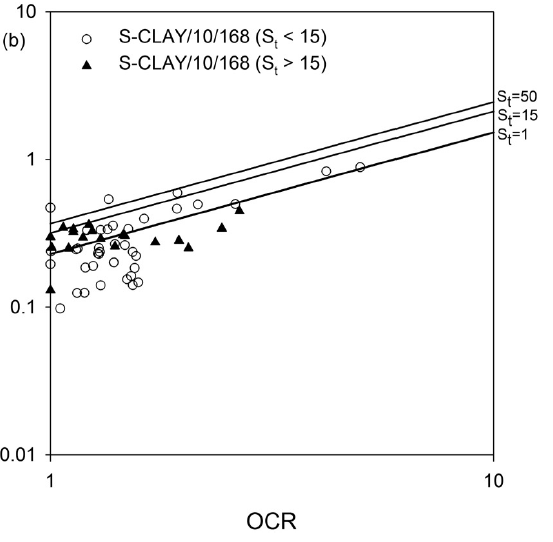
\includegraphics[width=0.48\textwidth]{figures/figure-6b.png}
        \label{figure:6b}
    }
\end{BiliFigure}
    \sidebyside[crosscolumn=true][p]{0.48\textwidth}{
    \begin{BiliFigure}[label=figure:7][H]{$\mathrm{LL}-\left(s_{\mathrm{u}}^{\mathrm{FV}} / \sigma_{\mathrm{p}}^{\prime}\right)$ model proposed by \citet{Hansbo1957}}{\citet{Hansbo1957}提出的$\mathrm{LL}-\left(s_{\mathrm{u}}^{\mathrm{FV}} / \sigma_{\mathrm{p}}^{\prime}\right)$模型}
        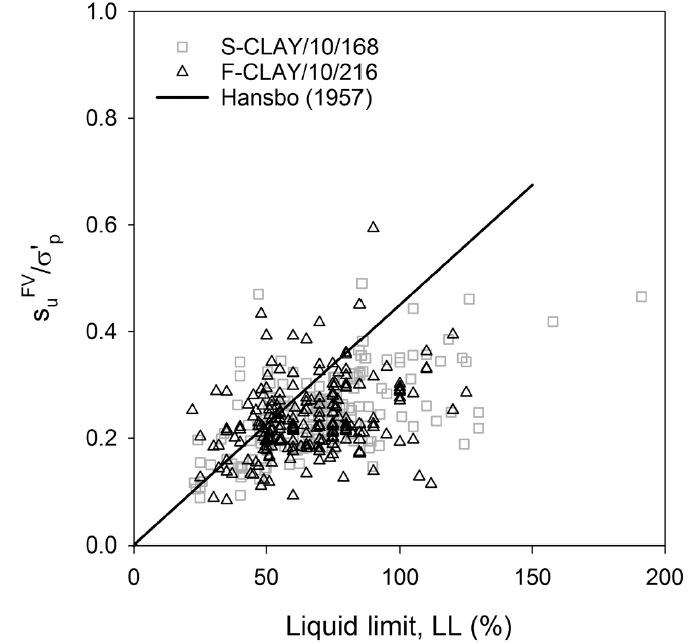
\includegraphics[width=\textwidth]{figures/figure-7.png}
    \end{BiliFigure}
}{0.48\textwidth}{
    \begin{BiliFigure}[label=figure:8][H]{$\mathrm{PI}-\left(s_{\mathrm{u}}^{\mathrm{FV}} / \sigma_{\mathrm{p}}^{\prime}\right)$ model proposed by \citet{Larsson1980591,Chandler198813}}{\citet{Larsson1980591,Chandler198813}提出的$\mathrm{PI}-\left(s_{\mathrm{u}}^{\mathrm{FV}} / \sigma_{\mathrm{p}}^{\prime}\right)$模型}
        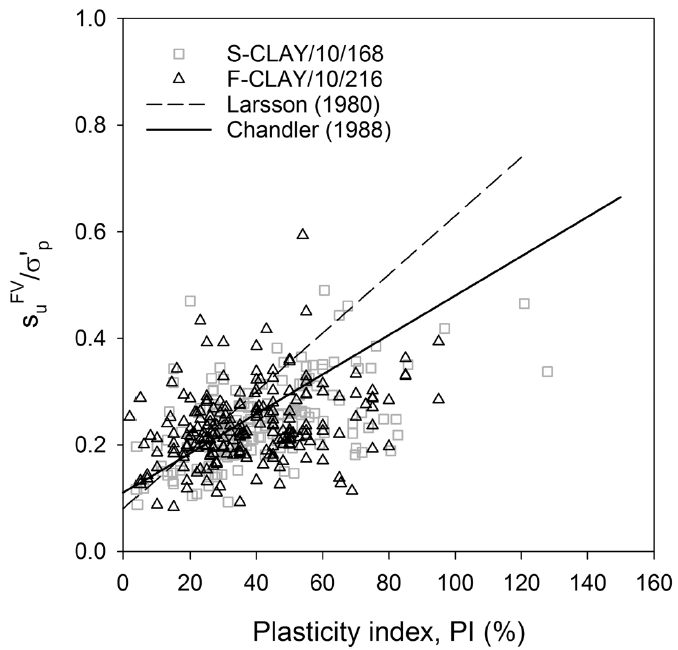
\includegraphics[width=\textwidth]{figures/figure-8.png}
    \end{BiliFigure}
}
    \sidebyside[crosscolumn=true][p]{0.48\textwidth}{
    \begin{BiliFigure}[label=figure:9][H]{$\mathrm{LI}-\left(s_{\mathrm{u}}^{\mathrm{re}} / P_{\mathrm{a}}\right)$ models}{$\mathrm{LI}-\left(s_{\mathrm{u}}^{\mathrm{re}} / P_{\mathrm{a}}\right)$模型}
        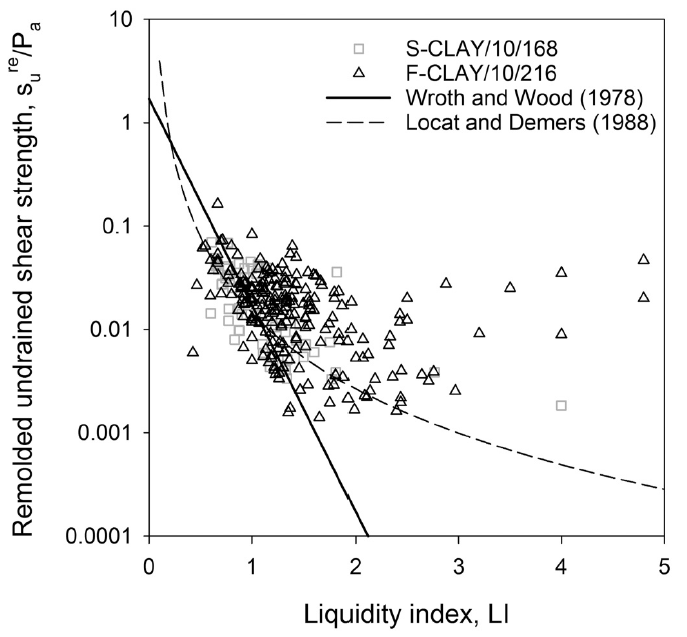
\includegraphics[width=\textwidth]{figures/figure-9.png}
    \end{BiliFigure}
}{0.48\textwidth}{
    \begin{BiliFigure}[label=figure:11][H]{$\mathrm{LI}-S_{\mathrm{t}}$ models}{$\mathrm{LI}-S_{\mathrm{t}}$模型}
        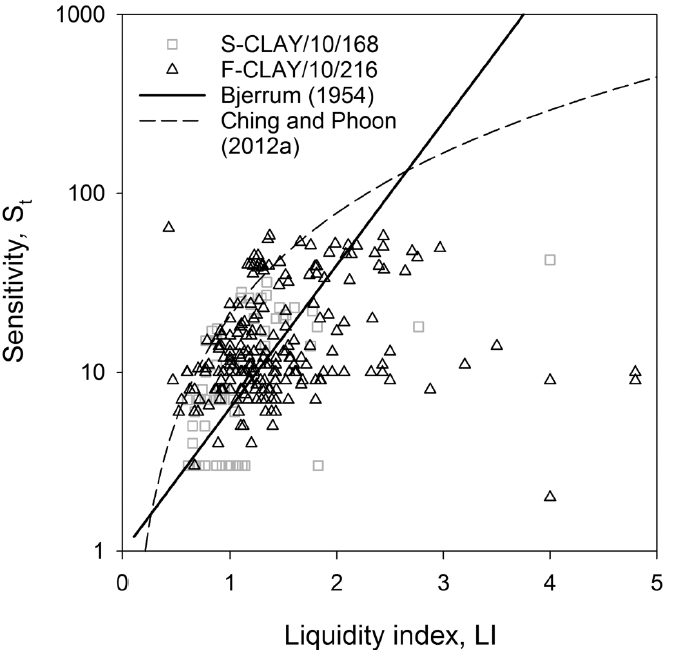
\includegraphics[width=\textwidth]{figures/figure-11.png}
    \end{BiliFigure}
}
    \begin{BiliFigure}[crosscolumn=true,label=figure:10][htb]{Comparison of strengths measured by FC, FV, and LVT}{通过FC,FV和LVT测量的强度比较}
    \subfigure[undisturbed]{
        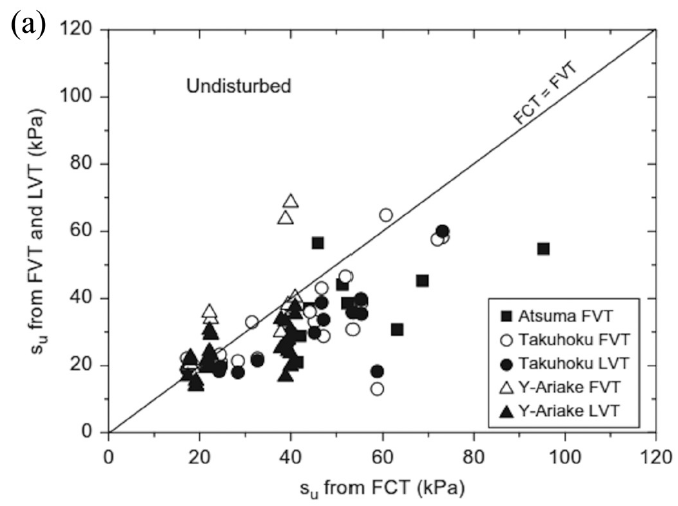
\includegraphics[width=0.48\textwidth]{figures/figure-10a.png}
        \label{figure:10a}
    }
    \hspace{\fill}
    \subfigure[remolded conditions \citep{Tanaka2012590}]{
        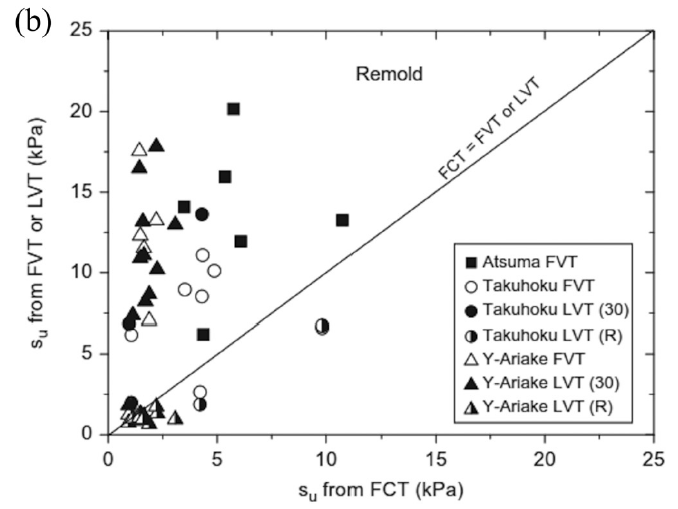
\includegraphics[width=0.48\textwidth]{figures/figure-10b.png}
        \label{figure:10b}
    }
\end{BiliFigure}

    \switchcolumn*
    
    \enautoref{figure:4}-\enautoref{figure:11} show the comparison between databases and transformation models. For the $\mathrm{LI}-\left(\sigma_{\mathrm{p}}^{\prime} / P_{\mathrm{a}}\right)-S_{\mathrm{t}}$ and $\mathrm{OCR}-\left[s_{\mathrm{u}}(\mathrm{mob}) / \sigma_{\mathrm{v}}^{\prime}\right]-S_{\mathrm{t}}$ models by \citet{Ching2012522}, data points are divided into two groups according to $S_t$ values. The two groups are based on the distinction between "low to medium sensitive" ($S_t<15$) and "highly sensitive" ($S_t>15$) clays suggested by \citet{Karlsrud20131273} for Norwegian clays.

    \switchcolumn

    \cnautoref{figure:4}-\cnautoref{figure:11}显示了数据库和转换模型之间的比较。 对于\citet{Ching2012522}的$\mathrm{LI}-\left(\sigma_{\mathrm{p}}^{\prime} / P_{\mathrm{a}}\right)-S_{\mathrm{t}}$和$\mathrm{OCR}-\left[s_{\mathrm{u}}(\mathrm{mob}) / \sigma_{\mathrm{v}}^{\prime}\right]-S_{\mathrm{t}}$模型,数据点根据$S_t$值被分为两组。 两组基于\citet{Karlsrud20131273}对挪威黏土提出的“中低敏感度”($S_t<15$)和“高敏感度”($S_t>15$)黏土的区别。

    \switchcolumn*

    The $\mathrm{OCR}-\left[s_{\mathrm{u}}(\mathrm{mob}) / \sigma_{\mathrm{v}}^{\prime}\right]$ transformation model by \citet{Jamiolkowski198557} provides a reasonable average fit to the data. For $\mathrm{OCR}<8$, $s_{\mathrm{u}}(\mathrm{mob}) / \sigma_{\mathrm{v}}^{\prime}$ seems to be strongly dependent on OCR (\enautoref{figure:4}). A deviation from the trend line in \enautoref{figure:4} is visible at OCR values greater than 5. However, data points with $\mathrm{OCR}>5$ belong to layers located in proximity of the ground surface (above 1.50 m) where the clay might be fissured and (or) partially saturated. Therefore, the interest for those points is limited, because the focus of this study is on intact clays.

    \switchcolumn

    \citet{Jamiolkowski198557}的$\mathrm{OCR}-\left[s_{\mathrm{u}}(\mathrm{mob}) / \sigma_{\mathrm{v}}^{\prime}\right]$转换模型。  提供了一个合理的平均拟合数据。 对于$\mathrm{OCR}<8$,$s_{\mathrm{u}}(\mathrm{mob}) / \sigma_{\mathrm{v}}^{\prime}$似乎与OCR密切相关(\cnautoref{figure:4})。 在OCR>5时,可以看到与\cnautoref{figure:4}中趋势线的偏离。但是,OCR>5的数据点属于位于地面附近(1.50 m以上)的层,黏土可能会开裂,且(或)部分饱和。因此,我们对这些观点的研究兴趣是有限的,因为本研究的重点是完整的黏土。

    \switchcolumn*

    The $\mathrm{PI}-\left[s_{\mathrm{u}}(\mathrm{mob}) / \sigma_{\mathrm{p}}^{\prime}\right]$ model by \citet{Mesri1975409,Mesri1989162} takes out the dependency of $s_{\mathrm{u}}(\mathrm{mob})$ on PI, stating that $s_{\mathrm{u}}(\mathrm{mob}) / \sigma_{\mathrm{p}}^{\prime}$ is constant and equal to 0.22. From \enautoref{figure:5}, $s_{\text {u }}$ (mob) $/ \sigma_{\text {p }}^{\prime}$ seems independent of PI, thus confirming the suggestion given by Mesri.

    \switchcolumn

    \citet{Mesri1975409,Mesri1989162}的$\mathrm{PI}-\left[s_{\mathrm{u}}(\mathrm{mob}) / \sigma_{\mathrm{p}}^{\prime}\right]$模型去除了$s_{\mathrm{u}}(\mathrm{mob})$对PI的依赖性,并指出$s_{\mathrm{u}}(\mathrm{mob}) / \sigma_{\mathrm{p}}^{\prime}$是常数且等于0.22。 从\cnautoref{figure:5}可以看出,$s_{\mathrm{u}}(\mathrm{mob}) / \sigma_{\mathrm{p}}^{\prime}$似乎与PI无关,从而证实了Mesri的建议。

    \switchcolumn*

    The dependency of $s_{\mathrm{u}}$ on $\mathrm{S}_{\mathrm{t}}$ predicted by the $\mathrm{OCR}-\left[s_{\mathrm{u}}(\mathrm{mob}) / \sigma_{\mathrm{v}}^{\prime}\right]-S_{\mathrm{t}}$ model by \citet{Ching2012522}, is not visible from the collected data points (\enautoref{figure:6}). However, the majority of the F-CLAY/10/216 data points for $S_{\mathrm{t}}<15$ are located between the $s_{\mathrm{u}}(\mathrm{mob}) / \sigma_{\mathrm{v}}^{\prime}-\mathrm{OCR}$ trend lines for $S_{\mathrm{t}}=1$ and $S_{\mathrm{t}}=15$ (\enautoref{figure:6a}).

    \switchcolumn

    从\citet{Ching2012522}的$\mathrm{OCR}-\left[s_{\mathrm{u}}(\mathrm{mob}) / \sigma_{\mathrm{v}}^{\prime}\right]-S_{\mathrm{t}}$模型所预测收集的数据点中看不到对$s_{\mathrm{u}}$对于$\mathrm{S}_{\mathrm{t}}$的依赖性(\cnautoref{figure:6})。 但是,$S_{\mathrm{t}}<15$的大多数F-CLAY/10/216数据点位于$S_{\mathrm{t}}=1$和$S_{\mathrm{t}}=15$的$s_{\mathrm{u}}(\mathrm{mob}) / \sigma_{\mathrm{v}}^{\prime}-\mathrm{OCR}$趋势线之间(\cnautoref{figure:6a})。

    \switchcolumn*

    It is quite difficult to observe a well-defined trend for the data points to the $\mathrm{LL}-\left(s_{\mathrm{u}}^{\mathrm{F}} / \sigma_{\mathrm{p}}^{\prime}\right)$ model by \citet{Hansbo1957} (\enautoref{figure:7}). Both databases seem to better adapt to the mean trend suggested by the $\mathrm{PI}-\left(s_{\mathrm{u}}^{\mathrm{FV}} / \sigma_{\mathrm{p}}^{\prime}\right)$ models (\enautoref{figure:8}), although high scatter can be observed along the trend lines suggested by \citet{Larsson1980591} and \citet{Chandler198813} (after \citet{Skempton195419}).

    \switchcolumn

    \citet{Hansbo1957}的$\mathrm{LL}-\left(s_{\mathrm{u}}^{\mathrm{F}} / \sigma_{\mathrm{p}}^{\prime}\right)$模型很难观察到一个指向的数据点的清晰的趋势(\cnautoref{figure:7})。尽管我们可以沿着\citet{Larsson1980591}和\citet{Chandler198813}(在\citet{Skempton195419}之后)提出的趋势线观察到数据点高度分散,但两个数据库似乎都更好地适应了$\mathrm{PI}-\left(s_{\mathrm{u}}^{\mathrm{FV}} / \sigma_{\mathrm{p}}^{\prime}\right)$模型建议的平均趋势(\cnautoref{figure:8})。

    \switchcolumn*

    Data points seem to depart from the $\mathrm{LI}-\left(s_{\mathrm{u}}^{\mathrm{re}} / P_{\mathrm{a}}\right)$ model by \citet{Wroth1978137} for LI values greater than 1 (\enautoref{figure:9}). However, the transformation model by \citet{Locat1988799} seems able to reproduce the trend observed for $\mathrm{LI}<2$ (\enautoref{figure:9}). For $\mathrm{LI}>2$, the data points deviate from the existing transformation models. The authors believe that $S_{\mathrm{t}}$ was determined from the FV test for some of the Finnish data points (from \citet{Gardemeister1973113}). The FV test is known to produce higher $s_{\mathrm{u}}^{\mathrm{re}}$ values than the conventional fall cone $(\mathrm{FC})$ test. \citet{Tanaka2012590} demonstrated how $s_{\mathrm{u}}^{\mathrm{re}}$ determined from the FV test and the laboratory vane test (LVT) is as much as tenfold larger than $s_{\mathrm{u}}^{\mathrm{re}}$ determined using the FC test (Fig. 10b). This was attributed to the different remolding methods, as the turning of the vane is not equivalent to the remolded state for the FC test, which is obtained by kneading by hand. Hence, the actual $s_{\mathrm{u}}^{\mathrm{re}}$ may be lower than that shown in Fig. 9, which consequently produces a higher $S_{\mathrm{t}}$.  However, there are only 29 points with $\mathrm{LI}>2$.  The conclusions of this study will be largely unaffected, because 29 points only constitute $13.4\%$ of the total number of points. Based on the experimental results presented by \citet{Tanaka2012590}, the authors would like to further suggest that while undisturbed $s_{\mathrm{u}}$ values from FV and FC can be mixed (as shown in \enautoref{figure:10a} ), $s_{\mathrm{u}}^{\mathrm{re}}$ or derived parameters ($S_{\mathrm{t}}$) between $\mathrm{FV}$ and $\mathrm{FC}$ should be treated separately (as suggested by \enautoref{figure:10b} ).

    \switchcolumn

    \citet{Wroth1978137}对于LI值大于1的数据点似乎偏离了$\mathrm{LI}-\left(s_{\mathrm{u}}^{\mathrm{re}} / P_{\mathrm{a}}\right)$模型(\cnautoref{figure:9})。 但是,\citet{Locat1988799}的转换模型似乎能够重现对于LI<2观察到的趋势(\cnautoref{figure:9})。 对于LI>2,数据点偏离现有的转换模型。 作者认为,$S_{\mathrm{t}}$是通过FV试验确定的一些芬兰数据点(来自\citet{Gardemeister1973113})。 已知FV试验会产生比传统的落锥(FC)试验更高的输出值。 \citet{Tanaka2012590}证明了通过FV试验确定的结果和实验室叶片试验(LVT)的结果是使用FC试验确定的结果的十倍之多(\cnautoref{figure:10b})。 这归因于不同的重塑方法,因为叶片的旋转不等同于通过手动捏合获得的FC试验的重塑状态。 因此,实际的结果可能会低于\cnautoref{figure:9}所示的结果,因此会产生更高的$S_{\mathrm{t}}$。但是,LI>2的数据点仅有29个。该研究的结论将在很大程度上不受影响,因为仅29个数据点占总数据点 的13.4$\%$。 基于\citet{Tanaka2012590}提出的实验结果,作者想进一步建议,尽管可以混合FV和FC的不受干扰的$s_{\mathrm{u}}$值(如\cnautoref{figure:10a}所示),但FV和FC之间的$s_{\mathrm{u}}^{\mathrm{re}}$或派生参数($S_{\mathrm{t}}$)应分开对待(如\cnautoref{figure:10b}建议)。

    \switchcolumn*

    The $\mathrm{LI}-\left(S_{\mathrm{t}}\right)$ model by \citet{Bjerrum195449} can reasonably describe the data points for $\mathrm{LI}<2$, despite the high scatter observed (\enautoref{figure:11}). In contrast, the global model by Ching and Phoon (2012a) seems to provide an upper bound rather than an average fit to the databases (\enautoref{figure:11}).

    \switchcolumn

    尽管观察到高度分散(\cnautoref{figure:11}),但\citet{Bjerrum195449}的$\mathrm{LI}-\left(S_{\mathrm{t}}\right)$模型可以合理地描述LI<2的数据点。 相比之下,\citet{Ching2012522}的全局模型似乎为数据库提供了上限,而不是平均拟合(\cnautoref{figure:11})。

    \switchcolumn*

    The $\mathrm{LI}-\left(\sigma_{p}^{\prime} / P_{a}\right)-S_{t}$ model by \citet{Ching2012522} does not seem to fit the data points in F-CLAY/10/216 for $S_t<15$ (\enautoref{figure:12a}). The $\mathrm{LI}-\left(\sigma_{\mathrm{p}}^{\prime} / \mathrm{P}_{\mathrm{a}}\right)-S_{\mathrm{t}}$ transformation model appears to provide a better description of the highly sensitive clays $\left(S_{\mathrm{t}}>15\right)$ in F-CLAY/10/216 as the majority of the points are contained in the interval between the $\mathrm{LI}-\left(\sigma_{\mathrm{p}}^{\prime} / P_{\mathrm{a}}\right)-S_{\mathrm{t}}$ lines for $S_{\mathrm{t}}=15$ and $\mathrm{S}_{\mathrm{t}}=50$ (\enautoref{figure:12a}). In contrast, for the low to medium sensitive clays $\left(S_{\mathrm{t}}<15\right)$ in S-CLAY/10/168, most of the data points are comprised between the $\mathrm{LI}-\left(\sigma_{\mathrm{p}}^{\prime} / \mathrm{P}_{\mathrm{a}}\right)-S_{\mathrm{t}}$ boundary lines for $S_{\mathrm{t}}=1$ and $S_{\mathrm{t}}=15$ (\enautoref{figure:12b}), while for the highly sensitive clays, the models cannot satisfactorily describe the observed values.

    \switchcolumn

    \citet{Ching2012522}提出的$\mathrm{LI}-\left(\sigma_{p}^{\prime} / P_{a}\right)-S_{t}$模型似乎不适合$S_t<15$的F-CLAY/10/216中的数据点(\cnautoref{figure:12a})。$\mathrm{LI}-\left(\sigma_{\mathrm{p}}^{\prime} / \mathrm{P}_{\mathrm{a}}\right)-S_{\mathrm{t}}$转换模型似乎可以更好地描述F-CLAY/10/216中的高敏感黏土($S_t>15$),因为大多数点都包含在$S_t=15$和$S_t=50$的$\mathrm{LI}-\left(\sigma_{\mathrm{p}}^{\prime} / P_{\mathrm{a}}\right)-S_{\mathrm{t}}$线之间(\cnautoref{figure:12a})。 相比之下,对于S-CLAY/10/168中的中低敏感度黏土($S_t<15$),对于,大多数数据点包含在$S_t=1$和$S_t=15$的$\mathrm{LI}-\left(\sigma_{\mathrm{p}}^{\prime} / \mathrm{P}_{\mathrm{a}}\right)-S_{\mathrm{t}}$边界线之间(\cnautoref{figure:12b}),而对于高度敏感的黏土,模型不能令人满意地描述观测值。

    \CrossColumnText{
        \begin{BiliFigure}[label=figure:12][htb]{$\mathrm{LI}-\left(\sigma_{\mathrm{p}}^{\prime}/\mathrm{P}_{\mathrm{a}}\right)-S_{\mathrm{t}}$ model by \citet{Ching2012522}}{\citet{Ching2012522}提出的$\mathrm{LI}-\left(\sigma_{\mathrm{p}}^{\prime}/\mathrm{P}_{\mathrm{a}}\right)-S_{\mathrm{t}}$模型}
    \subfigure[F-CLAY/10/216]{
        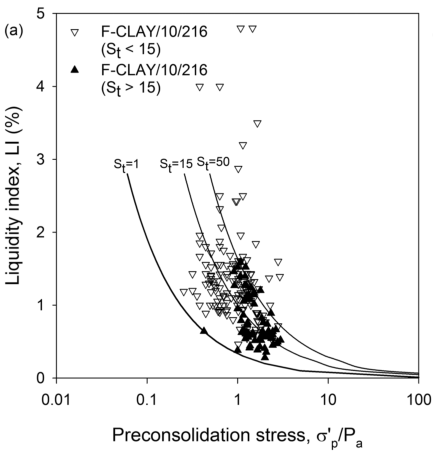
\includegraphics[width=0.48\textwidth]{figures/figure-12a.png}
        \label{figure:12a}
    }
    \hspace{\fill}
    \subfigure[S-CLAY/10/168]{
        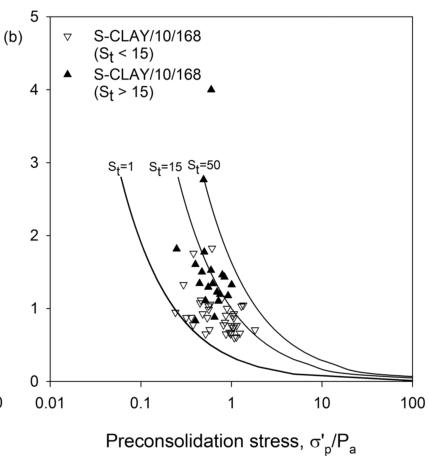
\includegraphics[width=0.48\textwidth]{figures/figure-12b.png}
        \label{figure:12b}
    }
\end{BiliFigure}
    }
    
    \switchcolumn*[\Paragraph{Bias and uncertainties of the existing transformation models 现有转换模型的偏差和不确定性}]

    Bias factor (denoted by $b$), and COV (denoted by $\delta$ ) are evaluated and discussed for the transformation models described in the previous section, based on the F-CLAY/10/216 and S-CLAY/10/168 databases. The parameters b and $\delta$ represent the sample mean and the COV, respectively, of the ratio (actual target value)/(predicted If $b=1,$ the model prediction is unbiased. For instance, for the $\mathrm{OCR}-\left[\mathrm{s}_{\mathrm{u}}(\mathrm{mob}) / \sigma_{\mathrm{v}}^{\prime}\right]$ transformation model by \citet{Jamiolkowski198557}, the actual target value is $s_{\mathbf{u}}(\mathrm{mob}) / \sigma_{\mathrm{v}}^{\prime}$ and the predicted target value is $0.23\mathrm{OCR}^{0.8}$. For the data points where $s_{\mathrm{u}}(\mathrm{mob}) / \sigma_{\mathrm{v}}^{\prime}$ and OCR are simultaneously known, (actual target value) (predicted target value) $=\left[s_{\mathrm{u}}(\mathrm{mob}) / \sigma_{\mathrm{v}}^{\prime}\right] /\left(0.23 \mathrm{OCR}^{0.8}\right)$.

    \switchcolumn

    在F-CLAY/10/216和S-CLAY/10/168数据库的基础上,针对上一节中描述的转换模型评估并讨论了偏差因子(以b表示)和COV(以$\delta$表示)。参数b和$\delta$分别代表比率(实际目标值)/(预测目标值)的样本平均值和COV。 如果$b = 1$,则模型预测是无偏的。 例如,对于\citet{Jamiolkowski198557}的$\mathrm{OCR}-\left[\mathrm{s}_{\mathrm{u}}(\mathrm{mob}) / \sigma_{\mathrm{v}}^{\prime}\right]$转换模型,实际目标值为$s_{\mathbf{u}}(\mathrm{mob}) / \sigma_{\mathrm{v}}^{\prime}$,预测目标值为$0.23\mathrm{OCR}^{0.8}$。 对于同时知道$s_{\mathrm{u}}(\mathrm{mob}) / \sigma_{\mathrm{v}}^{\prime}$和OCR的数据点,(实际目标值)/(预测的目标值)$=\left[s_{\mathrm{u}}(\mathrm{mob}) / \sigma_{\mathrm{v}}^{\prime}\right] /\left(0.23 \mathrm{OCR}^{0.8}\right)$。

    \switchcolumn*

    According to \citet{Ching2014663}:

    \switchcolumn

    根据\citet{Ching2014663}:

    \CrossColumnText{
        \begin{align}
            \varepsilon&=(\rm actual~target~value)/(b\times{}\rm predicted~target~value)\\
            &=(\rm actual~target~value)/(\rm unbiased~prediction)\nonumber
        \end{align}
    }

    \switchcolumn*

    \noindent
    where $\varepsilon$ is the variability term with mean = 1 and $\mathrm{COV}=\delta$. If $\delta=0$ there is no data scatter about the transformation model, indicating that the prediction is deterministic, rather than uncertain.

    \switchcolumn

    \noindent
    其中$\varepsilon$是mean = 1且$\mathrm{COV}=\delta$的变异项。 如果$\delta=0$,则转换模型没有数据分散,表明预测是确定性的而不是不确定的。

    \switchcolumn*

    Bias factors and COVs for the different transformation models analyzed are reported in \enautoref{table:6} for F-CLAY/10/216 and \enautoref{table:7} for S-CLAY/10/168, respectively. Bias factor, COV of $\varepsilon$, and number of data points used for each calibration are denoted, respectively, by $b$, $\delta$, and $n$.

    \switchcolumn

    \cnautoref{table:6}和\cnautoref{table:7}分别报告了F-CLAY/10/216和S-CLAY/10/168所分析的不同转换模型的偏差因子和COV。 偏差因子,$\varepsilon$的COV和每次校准所使用的数据点数分别由$b$,$\delta$和$n$表示。

    \CrossColumnText{
        \begin{table*}[!htb]
    \centering
    \footnotesize
    \caption{Transformation models for Finnish clays and their calibration results for S-CLAY/10/168.}
    \addtocounter{table}{-1}
    \vspace{-8pt}
    \renewcommand{\tablename}{表}
    \caption{芬兰黏土的转换模型及其S-CLAY/10/168的校准结果}
    \vspace{4pt}
    \renewcommand{\tablename}{Table}
    \setlength{\tabcolsep}{0.3mm}{
    \begin{tabular}{lllllllll}
        \toprule
                &                 &               &      &         & \multicolumn{2}{l}{Comprasion} & \multicolumn{2}{l}{Calibration} \\
        Type    & Relationship    & Literature    & $n$  & Transformation model & Figure & \makecell[l]{Fit to\\trend?} & \makecell{Bias\\factor,b} & \makecell{COV of\\$\varepsilon=\delta$}\\
        \midrule
        A       & \RelationshipAA & \LiteratureAA & 899  & \ModelAA &  Fig.\ref{figure:9}      & NO       & $-$        & $-$ \\
                &                 & \LiteratureAB & 899  & \ModelAB &  Fig.\ref{figure:9}      & YES      & 1.60      & 0.96 \\
                & \RelationshipAB & \LiteratureAC & 1279 & \ModelAC &  Fig.\ref{figure:11}     & YES      & 1.48      & 0.65 \\
                &                 & \LiteratureAD & 1279 & \ModelAD &  Fig.\ref{figure:11}     & NO       & 0.49      & 0.61 \\
        B       & \RelationshipBA & \LiteratureBA & 694  & \ModelBA &  Fig.\ref{figure:12}b    & YES      & 1.23      & 0.51 \\
                & \RelationshipBB & \LiteratureBB & 492  & \ModelBB &  Fig.\ref{figure:12}b    & YES      & 0.84      & 0.54 \\
        C       & \RelationshipCA & \LiteratureCA & 1072 & \ModelCA &  Fig.\ref{figure:5}      & YES      & 0.96      & 0.27 \\
                & \RelationshipCB & \LiteratureCB & 1155 & \ModelCB &  Fig.\ref{figure:6}      & YES      & 0.97      & 0.25 \\
                & \RelationshipCC & \LiteratureCC & 1402 & \ModelCC &  Fig.\ref{figure:6}b     & YES      & 0.71      & 0.36 \\
        D       & \RelationshipDA & \LiteratureDA & 423  & \ModelDA &  Fig.\ref{figure:7}      & YES      & 0.82      & 0.34 \\
                & \RelationshipDB & \LiteratureDB & 428  & \ModelDB &  Fig.\ref{figure:8}      & YES      & 0.85      & 0.37 \\
                &                 & \LiteratureDC & 423  & \ModelDC &  Fig.\ref{figure:8}      & YES      & 0.96      & 0.31 \\
        \bottomrule
    \end{tabular}}%
    \label{table:7}%
\end{table*}
    }
    \switchcolumn*

    The $\mathrm{LI}-\left(s_{\mathrm{u}}^{\mathrm{re}}/P_{\mathrm{a}}\right)$ model by \citet{Locat1988799} seems quite conservative, as it underpredicts the actual value by a factor of 4.05 for Finnish clays (\enautoref{table:6}) and 1.60 for Scandinavian clays (\enautoref{table:7}). \citet{Bjerrum195449} transformation model underestimates the actual $S_{\mathrm{t}}$ values for both Finnish and Scandinavian clays. Nevertheless, the uncertainty underlying these predictions still remains considerable, as the COV for type A models ranges between 61\% and 302\%. A similar analysis can be carried out for the $\mathrm{LI}-\left(\sigma_{\mathrm{p}}^{\prime}/P_{\mathrm{a}}\right)-S_{\mathrm{t}}$ model by \citet{Ching2012522}. The deviation of about $50\%-60\%$ from the mean trend lines of both F-CLAY/10/216 and S-CLAY/10/168, combined with a COV greater than 1 and equal to 0.61 for Finnish and Scandinavian clays, respectively, would result in predicted values characterized by a high degree of uncertainty. Therefore, models of type A and B are "biased" models with respect to both databases.

    \switchcolumn

    \citet{Locat1988799}提出的$\mathrm{LI}-\left(s_{\mathrm{u}}^{\mathrm{re}}/P_{\mathrm{a}}\right)$模型似乎很保守,因为它低估了芬兰黏土的实际价值(4.05)(\cnautoref{table:6})和斯堪的纳维亚黏土的1.60(\cnautoref{table:7})。\citet{Bjerrum195449}的转换模型低估了芬兰和斯堪的纳维亚黏土的实际$ S_{\mathrm{t}}$值。 但是,由于A型模型的COV在61$\%$至302$\%$之间,因此这些预测的不确定性仍然很大。\citet{Ching2012522}对$\mathrm{LI}-\left(\sigma_{\mathrm{p}}^{\prime}/P_{\mathrm{a}}\right)-S_{\mathrm{t}}$进行类似的分析。 与F-CLAY/10/216和S-CLAY/10/168的平均趋势线约为$50\%-60\%$的偏差,芬兰和斯堪的纳维亚的COV分别大于1和等于0.61,将导致以高度不确定性为特征的预测值。 因此,相对于两个数据库,类型A和B的模型都是“有偏差的”模型。

    \switchcolumn*

    In contrast, different outcomes are obtained for the transformation models of type C and D (models for shear strength). Models of type C ($s_{\mathrm{u}}(\mathrm{mob}) / \sigma_{\mathrm{v}}^{\prime}$ is the target parameter) show bias factors ($b$) close to 1 and COV ($\delta$) lower than 0.30. Exception is found for the $\mathrm{OCR}-\left[s_{\mathrm{u}}(\mathrm{mob}) / \sigma_{\mathrm{v}}^{\prime}\right]-S_{\mathrm{t}}$ model \citet{Ching2012522}, which shows a bias factor of 0.71-0.77 with a COV of 0.32-0.36. These results would thus suggest that $s_{\mathrm{u}}(\mathrm{mob})$ of Scandinavian clays can be described by different well established transformation models with relatively low uncertainty. For instance, the equation by Mesri (1975, 1989) can be adapted to Finnish soft clays by including the bias factor (b) calibrated from F-CLAY/10/216 database as $s_{\mathrm{u}}(\mathrm{mob})/\sigma_{\mathrm{p}}^{\prime}=b(0.22)=0.95(0.22)=0.209$, with a $\operatorname{COV}(\delta)=0.28(\mathrm{low}$ variability). 

    \switchcolumn

    相反,对于C型和D型转换模型(剪切强度模型)可获得不同的结果。 C型模型($s_{\mathrm{u}}(\mathrm{mob}) / \sigma_{\mathrm{v}}^{\prime}$是目标参数)显示偏差因子($b$)接近1而COV($\delta$)低于0.30。\citet{Ching2012522}提出的$\mathrm{OCR}-\left[s_{\mathrm{u}}(\mathrm{mob}) / \sigma_{\mathrm{v}}^{\prime}\right]-S_{\mathrm{t}}$模型中发现了例外,其偏差因子为0.71-0.77,COV为0.32-0.36。 因此,这些结果表明,斯堪的纳维亚黏土的$s_{\mathrm{u}}(\mathrm{mob})$可以用不确定性相对较低的各种完善的转化模型来描述。 例如,\citet{Mesri1975409,Mesri1989162}的方程可以通过引入F-CLAY/10/216数据库中校准的偏差因子($b$),$s_{\mathrm{u}}(\mathrm{mob})/\sigma_{\mathrm{p}}^{\prime}=b(0.22)=0.95(0.22)=0.209$, with a $\operatorname{COV}(\delta)=0.28$(低变异性)。
    
    \switchcolumn*

    Type D models ($s_{u}^{\mathrm{FV}}/\sigma_{\mathrm{p}}^{\prime}$ is the target parameter, see \enautoref{table:6}-\enautoref{table:7} show a bias factor $b$ varying between 0.82 and 0.97 with COV between 0.31 and 0.43, suggesting reasonably low variability for these models. In particular, the $\mathrm{PI}-\left(s_{\mathrm{u}}^{\mathrm{FV}}/\sigma_{\mathrm{p}}^{\prime}\right)$ model proposed by Chandler (1988) results almost "unbiased" with respect to both F-CLAY/10/216 and S-CLAY/10/168, suggesting $b$ comprised between 0.96-0.97 and $\delta$ varying between 0.31 and 0.35.

    \switchcolumn

    D型模型($s_{u}^{\mathrm{FV}}/\sigma_{\mathrm{p}}^{\prime}$是目标参数,请参见\cnautoref{table:6}-\cnautoref{table:7})显示偏置系数$b$在0.82和0.97之间变化,COV在0.31和0.43之间,表明这些模型的变异性较低。 特别是\citet{Chandler198813}提出的$\mathrm{PI}-\left(s_{\mathrm{u}}^{\mathrm{FV}}/\sigma_{\mathrm{p}}^{\prime}\right)$模型对于F-CLAY/10/216和S-CLAY/10/168几乎都是“无偏的”,表明$b$介于0.96-0.97,$\delta$在0.31和0.35之间变化。

\end{ParaColumn}